\documentclass[20pt]{beamer}

%% \usepackage{Boadilla}
\usepackage{tikz}
\usepackage{graphicx}

\title{Capable VMs:\\ Intro to CHERI}
\author{Jeremy Singer}
\date{20 Aug 2020}

\begin{document}

\begin{frame}
  
\includegraphics[width=3cm]{logo.png}
  \titlepage

\end{frame}

\begin{frame}
  \frametitle{What is a `capability'?}

  \begin{itemize}
  \item token of authority
  \item hardware supported permission descriptor
  \item fine-grained memory protection mechanism
  \end{itemize}
\end{frame}

\begin{frame}
  \frametitle{Capability replaces pointer}

  \begin{itemize}
  \item all mem accesses must be authorized by capability
  \item cap is double width of ptr; it includes:
    \begin{itemize}
    \item address
    \item 1-bit validity
    \item bounds info
    \item perms (r/w/x)
    \item other metadata
    \end{itemize}
  \end{itemize}
\end{frame}

\begin{frame}
  \frametitle{Enforced by Architecture}

  \begin{itemize}
  \item we cannot `fake' a capability
  \item we cannot change perms/bounds in a capability
  \end{itemize}
\end{frame}

\begin{frame}
  \frametitle{Architectural Extensions}
  CHERI generally bolted on to existing RISC ISA.
  \begin{itemize}
  \item extra data storage --- register file and memory tags
  \item extra instructions --- to manipulate capabilities and access memory through them
  \end{itemize}
\end{frame}

\begin{frame}
  \frametitle{Key uses for CHERI (1)}

  \begin{itemize}
  \item fine-grained memory protection in unsafe langs
    \begin{itemize}
       \item {\footnotesize like Valgrind only in hardware}
       \end{itemize}
     \end{itemize}
   \end{frame}

   \begin{frame}
  \frametitle{Key uses for CHERI (2)}
     \begin{itemize}
   \item software compartmentalization
        \begin{itemize}
        \item {\footnotesize Modern apps isolate components by running them in separate processes (with separate address spaces) --- high overhead}
        \item {\footnotesize with CHERI, we can isolate components within a single address space --- lower overhead}
          \item \emph{We want to do this for V8!}
    \end{itemize}

  \end{itemize}
  

\end{frame}


\begin{frame}
  \frametitle{CHERI Concept Stack}

  \begin{center}
  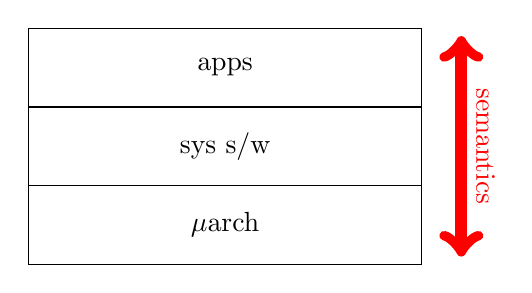
\begin{tikzpicture}
    \draw (0,0) rectangle (5,1) node[pos=.5] {$\mu$arch};
    \draw (0,1) rectangle (5,2) node[pos=.5] { sys s/w};
    \draw (0,2) rectangle (5,3) node[pos=.5] { apps };
    \draw[arrows=<->, line width=1.5mm, red](5.5,0.1)--(5.5,2.9) node[midway,above,rotate=-90] {semantics};
  \end{tikzpicture}
\end{center}

\end{frame}


\end{document}
